\begin{frame}{Многоквантовый эксперимент ЯМР\footnote[frame]{
J. Baum, M. Munowitz, A. N. Garroway, and A. Pines, J. Chem. Phys. 83, 2015 (1985).}}

  \begin{figure}
    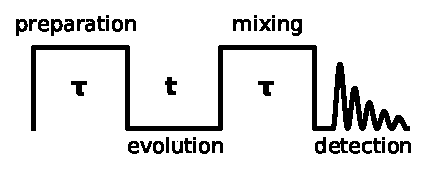
\includegraphics[width=0.5\textwidth]{mq-experiment-schema.pdf}
    %\caption{Схема МК эксперимента ЯМР}
  \end{figure}
  \vspace{-3mm}
  \begin{block}{}
    На подготовительном периоде МК эксперимента ЯМР система облучается последовательностью радиочастотных импульсов. В результате динамика спиновой системы определяется многоквантовым гамильтонианом.
    $$
    H_{MQ} = H^{(2)} + H^{(-2)},
    \quad H^{(\pm2)} = \frac 1 2 \sum_{i < j} D_{ij} I^\pm_i I^\pm_j
    $$
  \end{block}
\end{frame}
\note{
     МК динамику мы решили исследовать стандартным МК экспериментом.
     Эксперимент состоит из четырех частей,
     но нас будет интересовать только подготовительный период эксперимента.
     На подготовительном периоде ...слайд...
}

\begin{frame}{Многоквантовый экперимент ЯМР}
  \begin{columns}
    \column{0.4\textwidth}

    \begin{figure}
      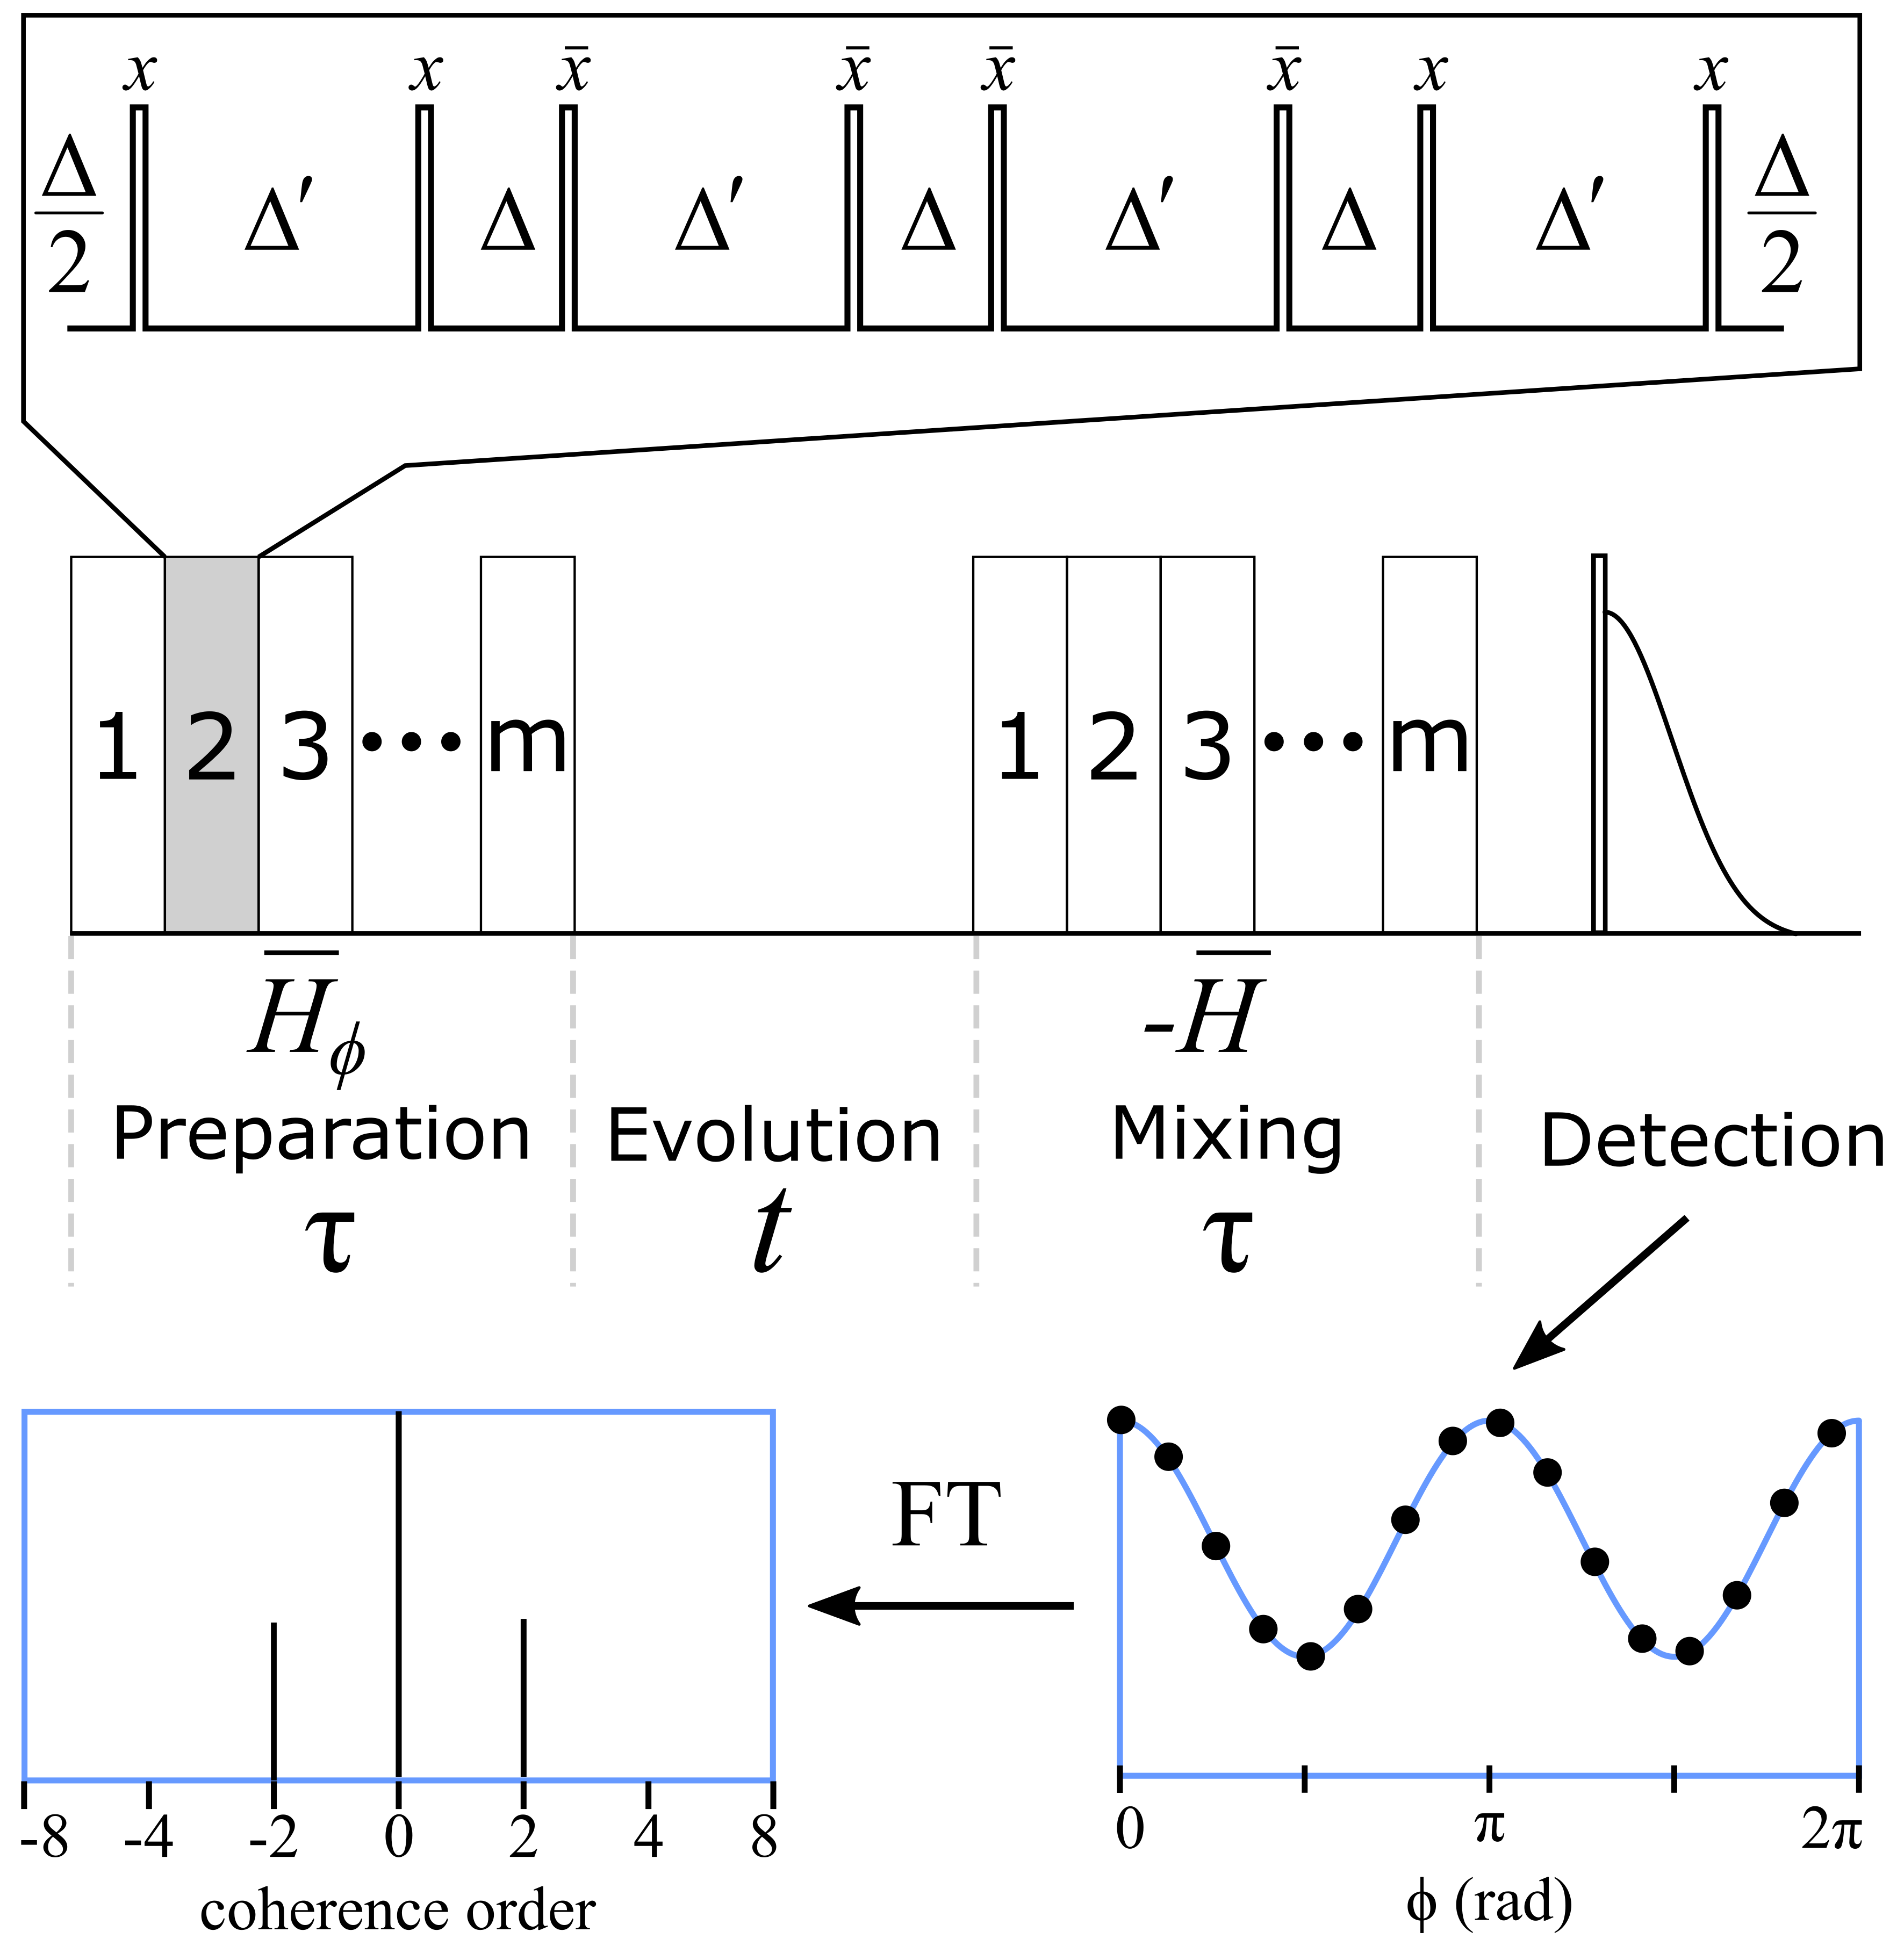
\includegraphics[width=0.9\textwidth]{mq-experiment-pulses-schema.png}
      \caption{Схематичное представление последовательности импульсов МК эксперимента.}
    \end{figure}


    \column{0.6\textwidth}
    МК когерентности создаются в течение периода подготовки продолжительностью $\tau$ при участии m-серии 8-импульсовых подпоследовательностей и затем преобразуются в наблюдаемую намагниченность после идентичного периода смешивания (за исключением 90-градусного фазового сдвига). Затем намагниченность детектируется при импульсе $\pi/2$. Фазовый сдвиг $\phi$ между периодами подготовки и смешивания инкриминируется для разделения многоквантовых когерентностей разных порядков. В результате преобразования Фурье по $\phi$ получается МК ЯМР спектр. Интенсивности МК когерентностей ЯМР при различных длительностях периода свободной эволюции $t$ получаются в отдельных экспериментах.
  \end{columns}
\end{frame}